\subsection{Cel dokumentu}\label{cel-dokumentu}

Niniejszy dokument ma na celu przestawienie wyników przeprowadzonych
analiz danych.

\subsection{Proste statystyki}\label{proste-statystyki}

Poniższa tabela przedstawia proste statystyki liczbowe dotyczące
zgromadzonych danych. Widzimy dysproporcję pomiędzy ilośćią danych
pochodzących z USA a ilością danych z Wielkiej Brytanii. Wynika z niej
podejście do analizy, w którym przeprowadzamy badania osobno na dancyh z
USA, osobno z Wielkiej Brytanii a następnie na danych połączonych.
Należy jednak mieć na uwadze, że dane połączone są mocno zdominowane
przez dane z USA.

\begin{longtable}[c]{@{}lllll@{}}
\toprule\addlinespace
Ilość danych & Wypadki & Pojazdy & Uczestniczący & Ofiary
\\\addlinespace
\midrule\endhead
USA & 1 300 141 & 1 947 730 & 3 430 324 & 1 450 505
\\\addlinespace
GB & 127 245 & 217 595 & 253 528 & 138 674
\\\addlinespace
\textbf{USA + GB} & \textbf{1 427 386} & \textbf{2 183 616} & \textbf{3
683 852} & \textbf{1 589 179}
\\\addlinespace
\bottomrule
\end{longtable}

\textbf{Analiza wypadków w czasie}

Dzień
tygodnia:\\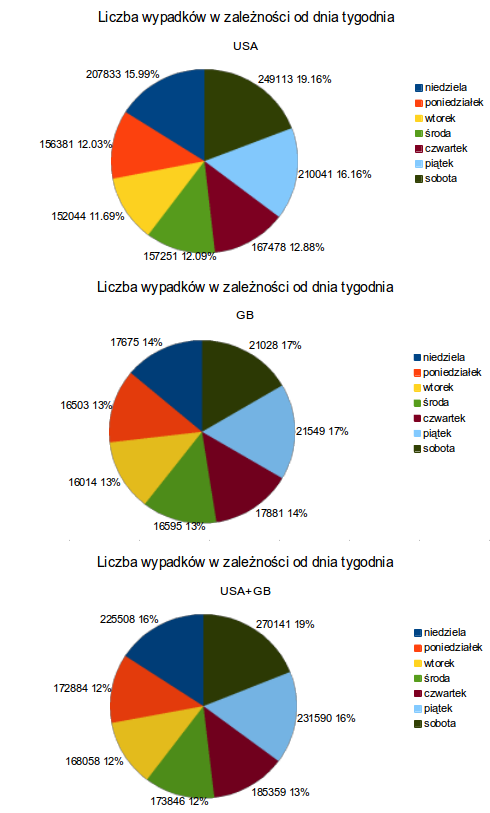
\includegraphics[width=0.8\textwidth]{images/statistics/day_of_week.png}

Rok:\\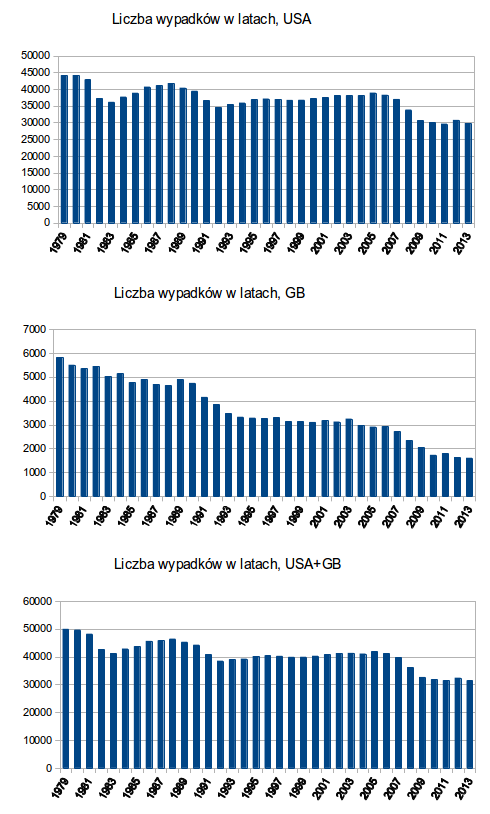
\includegraphics[width=0.8\textwidth]{images/statistics/year.png}

Miesiąc:\\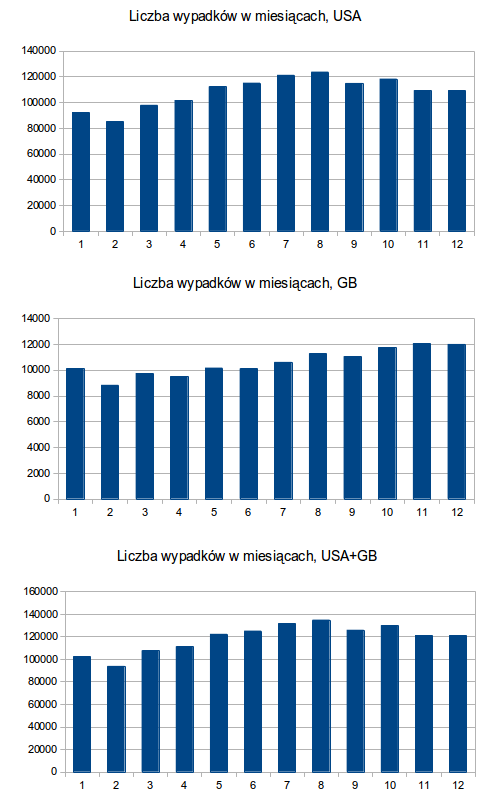
\includegraphics[width=0.8\textwidth]{images/statistics/month.png}

Dzień:\\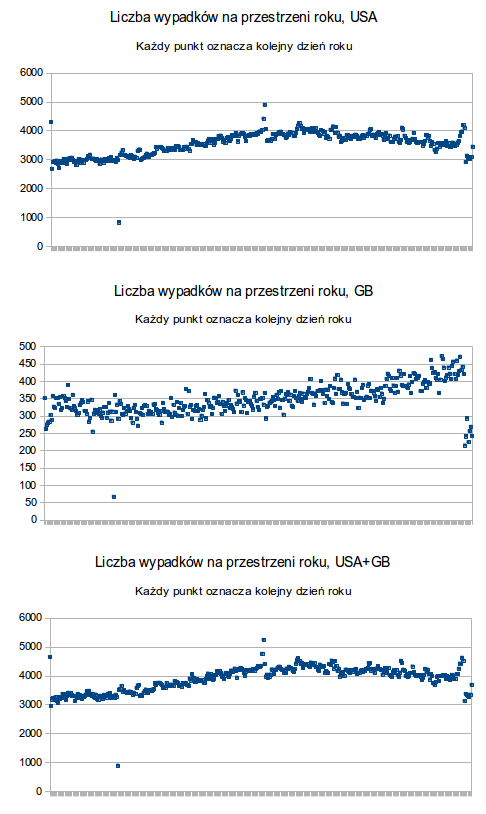
\includegraphics[width=0.8\textwidth]{images/statistics/day_of_year.png}

Bardzo niska wartość jest dla 29.02 - występuje tylko w latach
przestępnych i istotnie jest to wartość średnio 4 razy mniejsza.

Lokalne ``piki'' - \textbf{USA}:

\begin{itemize}
\itemsep1pt\parskip0pt\parsep0pt
\item
  01.01\\
\item
  03.07\\
\item
  04.07\\
\item
  02.08\\
\item
  03.08\\
\item
  31.10\\
\item
  01.11\\
\item
  20.12\\
\item
  21.12\\
\item
  22.12\\
\item
  23.12\\
\item
  24.12\\
\item
  31.12
\end{itemize}

Lokalne ``piki'' - \textbf{GB}:

\begin{itemize}
\itemsep1pt\parskip0pt\parsep0pt
\item
  21.01\\
\item
  01.03\\
\item
  18.04\\
\item
  01.05\\
\item
  15.08\\
\item
  07.09\\
\item
  20.10\\
\item
  30.10\\
\item
  05.12\\
\item
  21.12
\end{itemize}

Ciekawy jest spadek liczby wypadków w ostatnich dniach roku -
spowodowany prawdopodobnie faktem, że w tym okresie znacznie mniej osób
jeździ do pracy i spędza więcej czasu w domu z rodziną.

Godzina:\\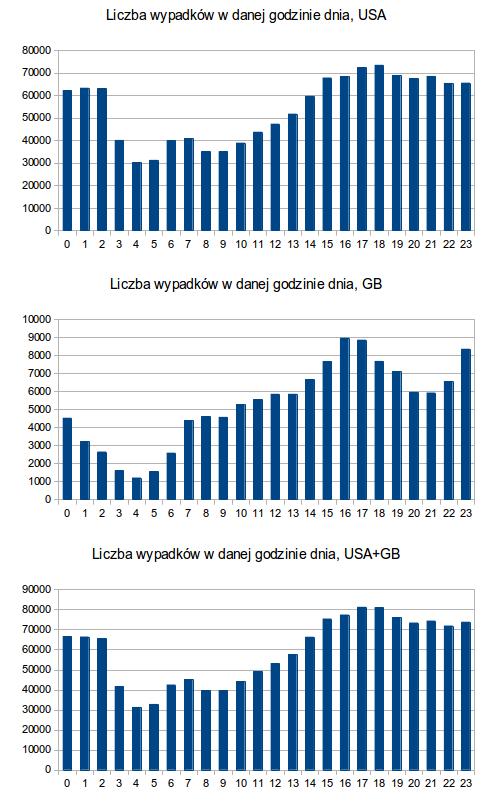
\includegraphics[width=0.8\textwidth]{images/statistics/hour.png}

\textbf{Ograniczenie prędkości}

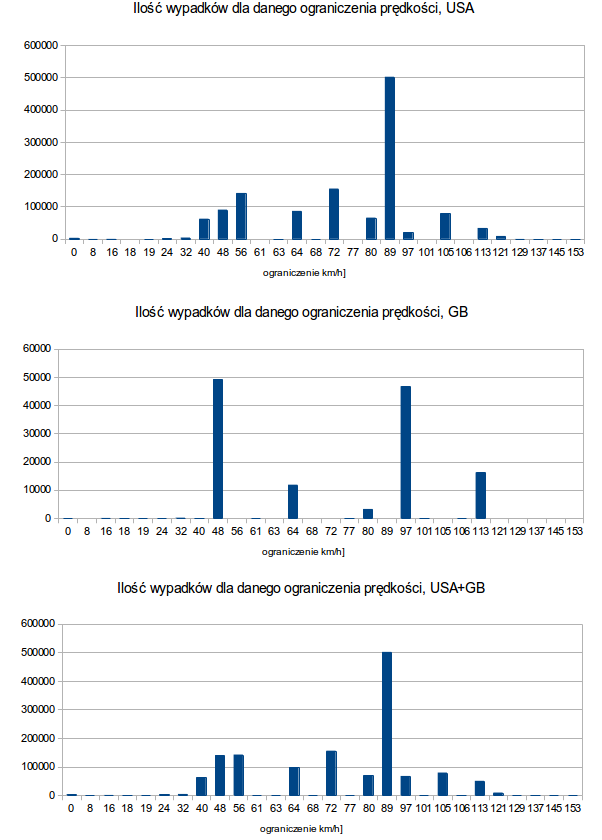
\includegraphics[width=0.8\textwidth]{images/statistics/speed_limit.png}

\textbf{Wiek kierowcy}

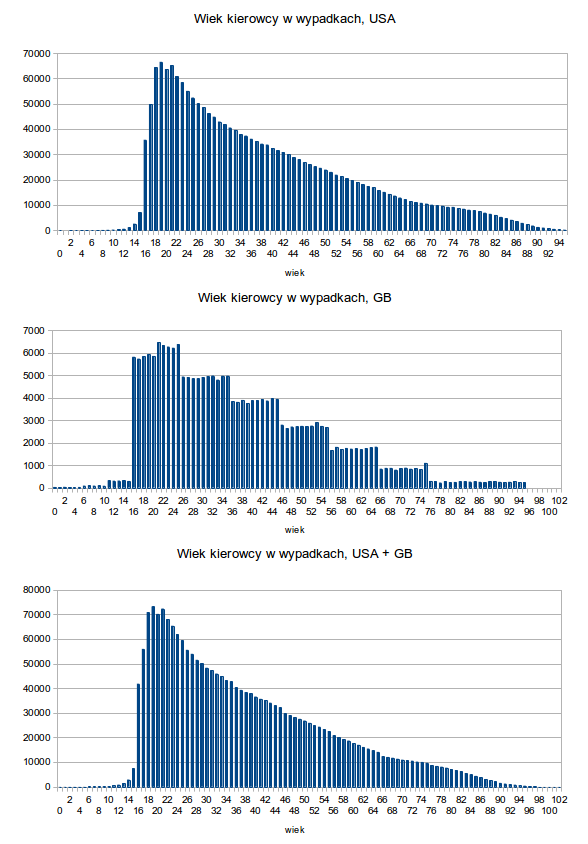
\includegraphics[width=0.8\textwidth]{images/statistics/driver_age.png}

\textbf{Wiek uczestników wypadku}

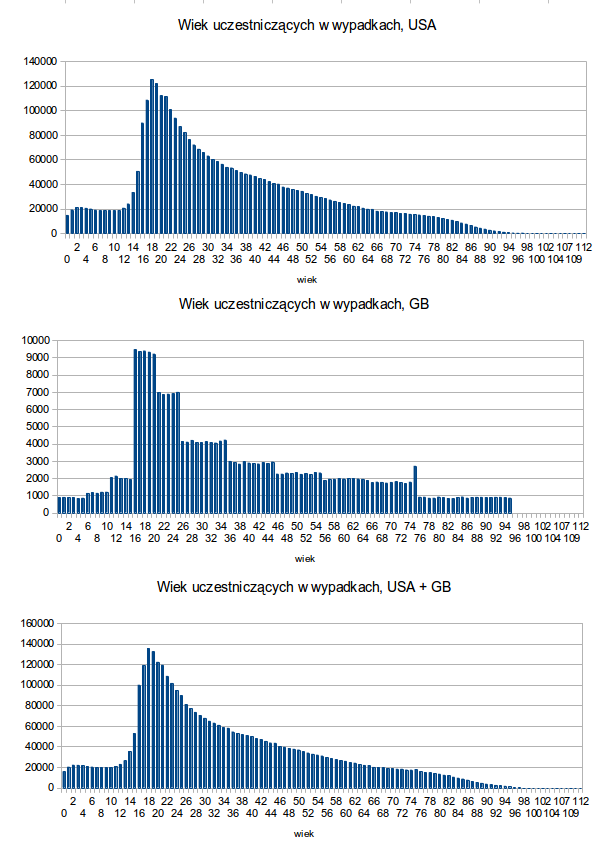
\includegraphics[width=0.8\textwidth]{images/statistics/person_age.png}

\textbf{Kierowcy pod wpływem alkoholu}

Dane o obecności alkoholu we krwi kierowcy są dostępne jedynie dla
danych z USA.

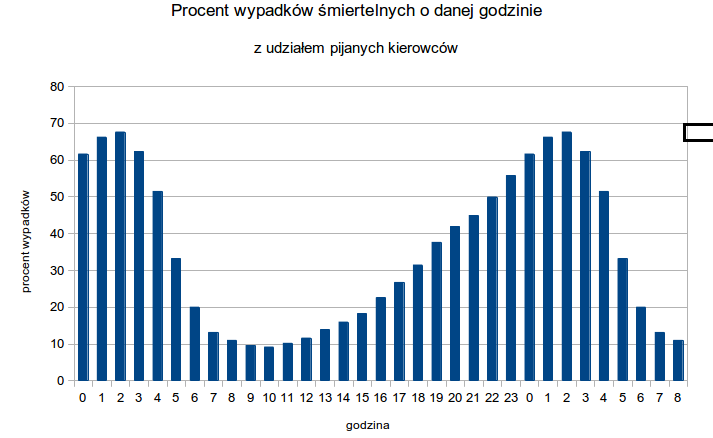
\includegraphics[width=0.8\textwidth]{images/hipotheses/drunk_drivers/hour.png}

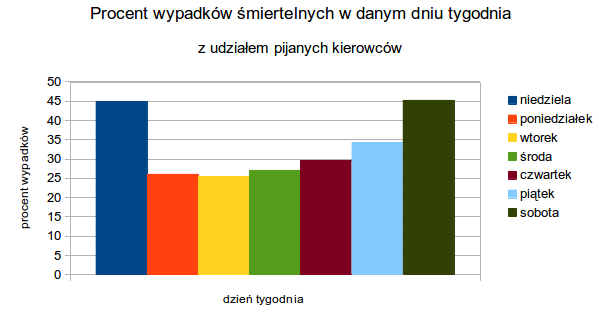
\includegraphics[width=0.8\textwidth]{images/hipotheses/drunk_drivers/day_of_week.png}

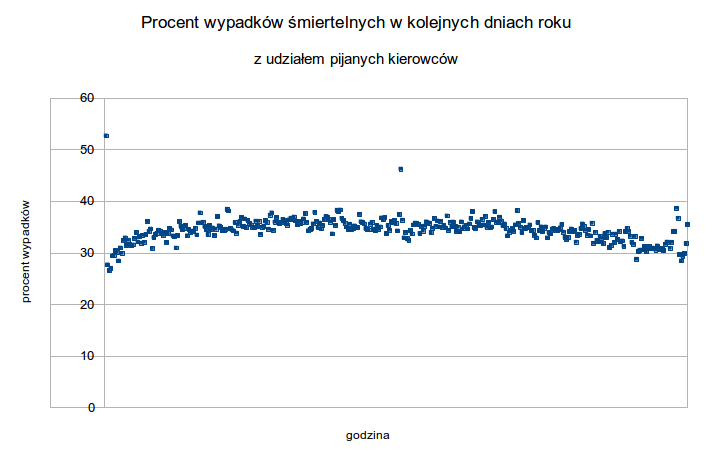
\includegraphics[width=0.8\textwidth]{images/hipotheses/drunk_drivers/day_of_year.png}

\textbf{Warunki pogodowe}\\Udział wypadków z różnymi kombinacjami
warunków pogodowych\\S - Snow\\W - Wind\\R - Rain\\F - Fog

\begin{longtable}[c]{@{}lllllll@{}}
\toprule\addlinespace
CONDS & USA & USA \% & GB & GB \% & USA+GB & USA+GB \%
\\\addlinespace
\midrule\endhead
NONE & 1142653 & 88,17\% & 104834 & 82,98\% & 1247487 & 87,71\%
\\\addlinespace
F & 17222 & 1,33\% & 1306 & 1,03\% & 18528 & 1,30\%
\\\addlinespace
W & 445 & 0,03\% & 2798 & 2,21\% & 3243 & 0,23\%
\\\addlinespace
WF & 2 & 0,00\% & 0 & 0,00\% & 2 & 0,00\%
\\\addlinespace
R & 108652 & 8,38\% & 14463 & 11,45\% & 123115 & 8,66\%
\\\addlinespace
RF & 1444 & 0,11\% & 0 & 0,00\% & 1444 & 0,10\%
\\\addlinespace
RW & 65 & 0,01\% & 2177 & 1,72\% & 2242 & 0,16\%
\\\addlinespace
RWF & 0 & 0,00\% & 0 & 0,00\% & 0 & 0,00\%
\\\addlinespace
S & 19108 & 1,47\% & 565 & 0,45\% & 19673 & 1,38\%
\\\addlinespace
SF & 7 & 0,00\% & 0 & 0,00\% & 7 & 0,00\%
\\\addlinespace
SW & 2005 & 0,15\% & 191 & 0,15\% & 2196 & 0,15\%
\\\addlinespace
SWF & 6 & 0,00\% & 0 & 0,00\% & 6 & 0,00\%
\\\addlinespace
SR & 4283 & 0,33\% & 0 & 0,00\% & 4283 & 0,30\%
\\\addlinespace
SRF & 12 & 0,00\% & 0 & 0,00\% & 12 & 0,00\%
\\\addlinespace
SRW & 78 & 0,01\% & 0 & 0,00\% & 78 & 0,01\%
\\\addlinespace
SRWF & 0 & 0,00\% & 0 & 0,00\% & 0 & 0,00\%
\\\addlinespace
\bottomrule
\end{longtable}

\textbf{Prędkość}

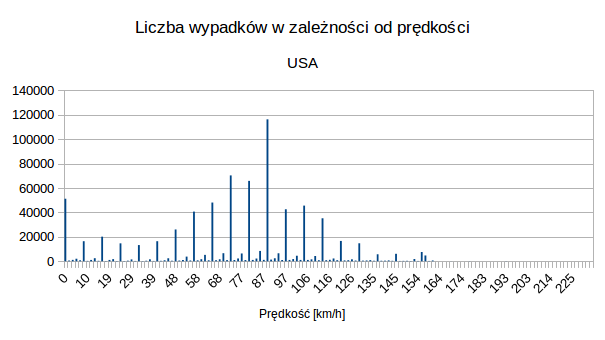
\includegraphics[width=0.8\textwidth]{images/hipotheses/speed/speed.png}

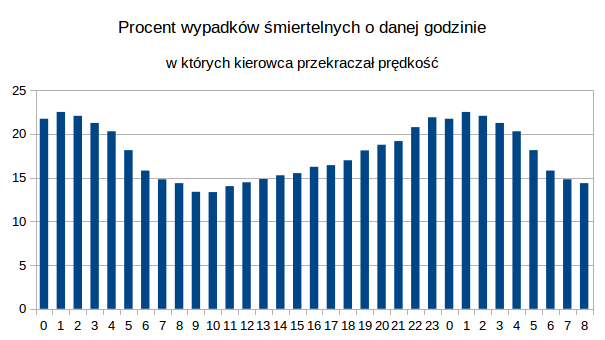
\includegraphics[width=0.8\textwidth]{images/hipotheses/speed/speed_exceeded_by_hour.png}

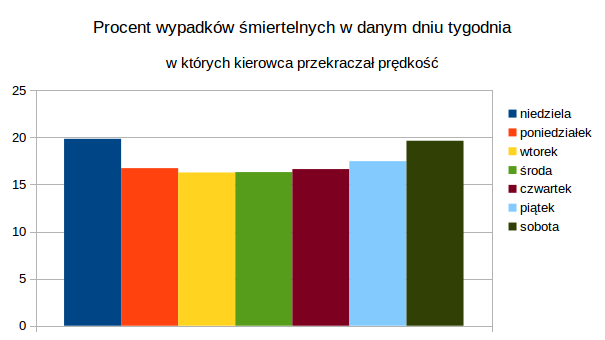
\includegraphics[width=0.8\textwidth]{images/hipotheses/speed/speed_exceeded_by_day_of_week.png}

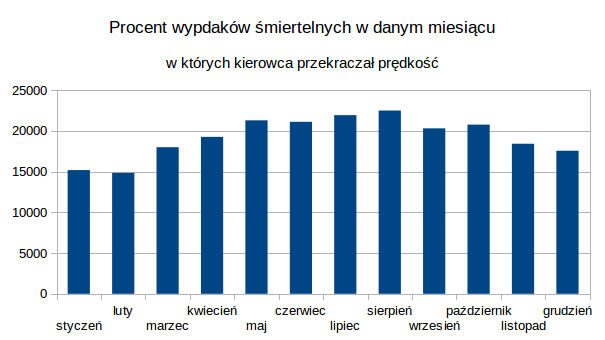
\includegraphics[width=0.8\textwidth]{images/hipotheses/speed/speed_exceeded_by_month.png}

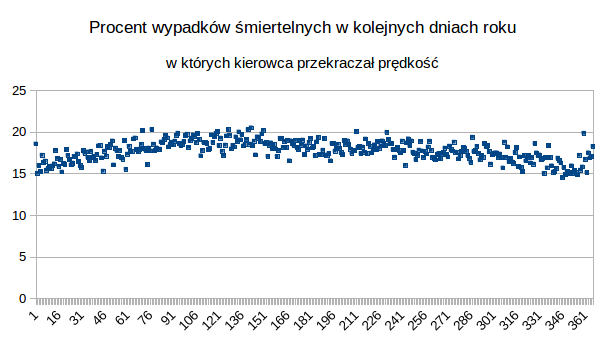
\includegraphics[width=0.8\textwidth]{images/hipotheses/speed/speed_exceeded_by_day_of_year.png}

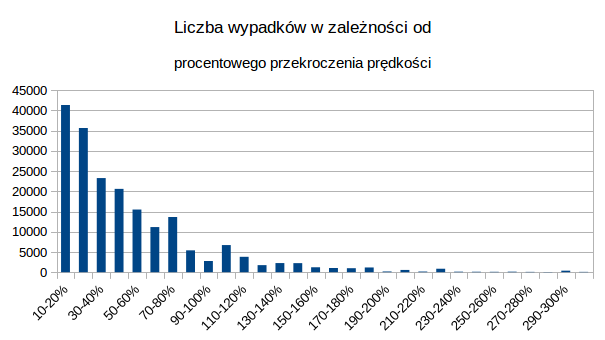
\includegraphics[width=0.8\textwidth]{images/hipotheses/speed/speed_exceeded_by_percent.png}

\textbf{Oświetlenie}

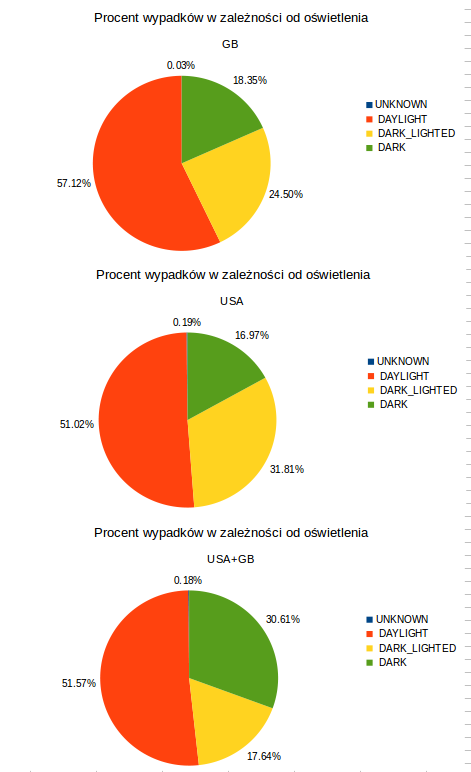
\includegraphics[width=0.8\textwidth]{images/hipotheses/lighting/lighting.png}

\textbf{Rodzaj drogi}

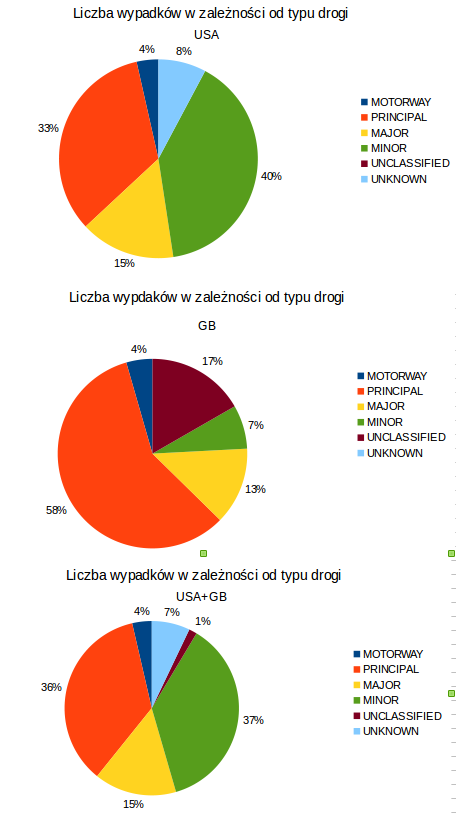
\includegraphics[width=0.8\textwidth]{images/statistics/road_type.png}

\textbf{Piesi}

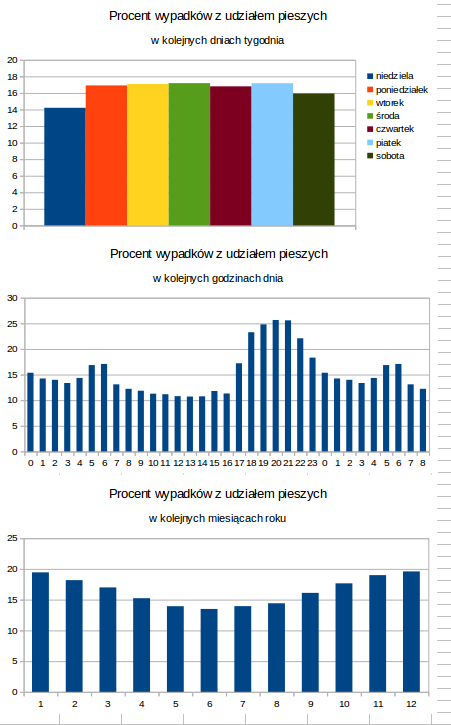
\includegraphics[width=0.8\textwidth]{images/hipotheses/pedestrians/pedestrians.png}

Wypadki z udziałem pieszych w warunkach ograniczających widoczność.

\begin{longtable}[c]{@{}ll@{}}
\toprule\addlinespace
warunki & procent
\\\addlinespace
\midrule\endhead
wszystkie & 16.36
\\\addlinespace
deszcz & 17.10
\\\addlinespace
śnieg & 10.37
\\\addlinespace
mgła & 13.72
\\\addlinespace
ciemność & 21.51
\\\addlinespace
\bottomrule
\end{longtable}
